% Appendix G: Cross-Task Analysis

\section{Cross-Task Analysis}
\label{app:cross_task_analysis}

This appendix provides the complete cross-task data underlying the comparisons in \S4.
All results use Qwen2.5-Coder-7B ($L{=}28$) unless stated otherwise.

%% ========== G.1 ==========
\subsection{Outcome Fingerprints: Full Data}
\label{app:subsec:outcome_fingerprints_full}

\cref{tab:app:outcome_fingerprint_full} reports the aggregate outcome distributions with per-task commentary on dominant failure modes.

\begin{table*}[t]
\centering
\caption{Full outcome fingerprints for Qwen2.5-Coder-7B across all six task families, with per-task commentary on failure characteristics.
Res.\ = Resolved, OT = Overprocessed, MR = Misresolved, UR = Unresolved.}
\label{tab:app:outcome_fingerprint_full}
\resizebox{\textwidth}{!}{%
\begin{tabular}{lrccccp{5.8cm}}
\toprule
Task & $N$ & Res.\% & OT\% & MR\% & UR\% & Commentary \\
\midrule
Pure Copying & 200 & 79.0 & 21.0 & 0.0 & 0.0 &
No MR or UR: the model always converges, but 21\% of samples are overprocessed---late layers corrupt a once-correct trace. \\
Computing & 207 & 33.5 & 45.9 & 12.4 & 8.1 &
Uniquely difficult: all four outcomes present in substantial proportions. Overprocessed dominates (45.9\%), yet it is the only task with notable MR (12.4\%) and UR (8.1\%), indicating qualitatively different failure modes. \\
Loop Unrolled & 298 & 89.3 & 8.1 & 2.7 & 0.0 &
Near-zero UR: the model always forms a convergence point. Residual MR (2.7\%) arises at high iteration counts. \\
Loop & 408 & 84.8 & 10.8 & 3.9 & 0.5 &
Similar to Loop Unrolled but with slightly elevated OT and a small UR fraction (0.5\%), syntactic loop structure adds marginal processing difficulty. \\
Conditional & 542 & 82.7 & 11.4 & 4.4 & 1.5 &
OT and MR rise together at high nesting depths; UR appears only at depth 3, indicating that deeply nested branches occasionally prevent convergence entirely. \\
Short-circuit & 346 & 86.1 & 10.4 & 3.5 & 0.0 &
Zero UR across all difficulty levels: the model always commits to an answer. Failures are exclusively OT or MR, consistent with the binary nature of short-circuit evaluation. \\
\midrule
Weighted avg. & 2001 & 79.2 & 15.1 & 4.3 & 1.3 & --- \\
\bottomrule
\end{tabular}%
}
\end{table*}

\paragraph{Computing as the sole four-way outlier.}
Computing is the only task where all four outcomes appear in substantial proportions.
The remaining five tasks share a common signature: Resolved $>$ 79\%, Overprocessed as the primary failure mode (8--21\%), and Misresolved and Unresolved together below 6\%.


%% ========== G.2 ==========
\subsection{Computing Density Sweep}
\label{app:subsec:computing_density_sweep}

The Computing task has two orthogonal difficulty axes: compute density $\rho \in \{0, 0.5, 1.0\}$ (fraction of steps requiring arithmetic) and chain length (steps $\in \{2,3,4,5\}$).
We sweep each independently.

\paragraph{Compute density ($\rho$) sweep.}

\cref{tab:app:rho_sweep} reports outcome distributions and mean brewing duration as $\rho$ increases.

\begin{table}[H]
\centering
\caption{Outcome distribution and mean brewing duration ($\Delta_{\mathrm{brew}}$) as a function of compute density $\rho$ for the Computing task (Qwen2.5-Coder-7B, pooled over all chain lengths).}
\label{tab:app:rho_sweep}
\resizebox{\columnwidth}{!}{%
\begin{tabular}{crccccc}
\toprule
$\rho$ & $N$ & Res.\% & OT\% & MR\% & UR\% & $\overline{\Delta}_{\mathrm{brew}}$ \\
\midrule
0   & 525 & 40.0 & 45.1 & 12.2 & 2.7 & 17.9 \\
0.5 & 309 & 19.7 & 23.6 & 30.1 & 26.5 & 13.4 \\
1.0 & 201 & 16.4 & 17.9 & 26.9 & 38.8 & 8.6 \\
\bottomrule
\end{tabular}%
}
\end{table}

\paragraph{Failure mode shift with arithmetic density.}
Even at $\rho{=}0$, the Resolved rate is lower than structurally similar control-flow tasks; multi-hop variable tracking itself is a bottleneck.
As $\rho$ increases, the failure character shifts: OT dominates at $\rho{=}0$, whereas MR and UR grow disproportionately at $\rho{=}1.0$, indicating that arithmetic demands \textbf{change the failure mechanism} from late-layer corruption to inability to reach the correct answer.
The brewing duration $\overline{\Delta}_{\mathrm{brew}}$ also contracts, consistent with the probe detecting partial (but incorrect) information earlier.

\paragraph{Chain length (steps) sweep.}

\cref{tab:app:step_sweep} isolates the effect of chain length.

\begin{table}[H]
\centering
\caption{Outcome distribution and layer-position statistics as a function of chain length (steps) for the Computing task (Qwen2.5-Coder-7B, pooled over all $\rho$).}
\label{tab:app:step_sweep}
\resizebox{\columnwidth}{!}{%
\begin{tabular}{crcccccc}
\toprule
Steps & $N$ & Res.\% & OT\% & MR\% & UR\% & $\overline{\mathrm{FPCL}}$ & $\overline{\mathrm{FJC}}$ \\
\midrule
2 & 260 & 48 & 38 & 8 & 6 & 7 & 20 \\
3 & 260 & 35 & 40 & 14 & 11 & 9 & 21 \\
4 & 260 & 24 & 42 & 18 & 16 & 10 & 21 \\
5 & 260 & 18 & 44 & 20 & 18 & 11 & 21 \\
\bottomrule
\end{tabular}%
}
\end{table}

\paragraph{Chain length as independent difficulty factor.}
Increasing chain length degrades outcomes even within fixed $\rho$ strata, demonstrating that sequential depth is an independent difficulty factor.
FPCL shifts later with longer chains while FJC remains stable, compressing the brewing window $\Delta_{\mathrm{brew}}$---mirroring the $\rho$-sweep pattern.


%% ========== G.3 ==========
\subsection{Per-Difficulty-Level Breakdown}
\label{app:subsec:per_difficulty_breakdown}

\cref{tab:app:per_difficulty_outcome} provides the complete per-difficulty-level outcome breakdown for all six task families.

\begin{table*}[t]
\centering
\caption{Per-difficulty-level outcome distributions for all six task families on Qwen2.5-Coder-7B.
Difficulty parameter varies by task: \emph{steps} for Copying and Computing (the latter at $\rho{=}1.0$), \emph{depth} for Conditional, \emph{num\_conditions} for Short-circuit, and \emph{iteration} for Loop and Loop Unrolled.}
\label{tab:app:per_difficulty_outcome}
\resizebox{\textwidth}{!}{%
\begin{tabular}{llrcccc}
\toprule
Task & Difficulty & $N$ & Res.\% & OT\% & MR\% & UR\% \\
\midrule
\multirow{5}{*}{Copying}
 & steps = 1 & 40 & 95.0 & 5.0 & 0.0 & 0.0 \\
 & steps = 2 & 40 & 87.5 & 12.5 & 0.0 & 0.0 \\
 & steps = 3 & 40 & 77.5 & 22.5 & 0.0 & 0.0 \\
 & steps = 4 & 40 & 72.5 & 27.5 & 0.0 & 0.0 \\
 & steps = 5 & 40 & 62.5 & 37.5 & 0.0 & 0.0 \\
\midrule
\multirow{4}{*}{Computing ($\rho{=}1.0$)}
 & steps = 2 & 51 & 33.3 & 23.5 & 17.6 & 25.5 \\
 & steps = 3 & 50 & 18.0 & 20.0 & 26.0 & 36.0 \\
 & steps = 4 & 50 & 10.0 & 16.0 & 30.0 & 44.0 \\
 & steps = 5 & 50 & 4.0 & 12.0 & 34.0 & 50.0 \\
\midrule
\multirow{3}{*}{Conditional}
 & depth = 1 & 196 & 98.0 & 2.0 & 0.0 & 0.0 \\
 & depth = 2 & 190 & 83.2 & 13.7 & 3.2 & 0.0 \\
 & depth = 3 & 156 & 62.8 & 20.5 & 11.5 & 5.1 \\
\midrule
\multirow{3}{*}{Short-circuit}
 & num\_cond = 1 & 72 & 100.0 & 0.0 & 0.0 & 0.0 \\
 & num\_cond = 2 & 134 & 83.6 & 10.4 & 6.0 & 0.0 \\
 & num\_cond = 3 & 140 & 81.4 & 15.7 & 2.9 & 0.0 \\
\midrule
\multirow{4}{*}{Loop}
 & iteration = 1 & 160 & 97.5 & 2.5 & 0.0 & 0.0 \\
 & iteration = 2 & 88 & 56.8 & 36.4 & 6.8 & 0.0 \\
 & iteration = 3 & 90 & 80.0 & 8.9 & 8.9 & 2.2 \\
 & iteration = 4 & 70 & 97.1 & 0.0 & 2.9 & 0.0 \\
\midrule
\multirow{4}{*}{Loop Unrolled}
 & iteration = 1 & 80 & 90.0 & 10.0 & 0.0 & 0.0 \\
 & iteration = 2 & 80 & 100.0 & 0.0 & 0.0 & 0.0 \\
 & iteration = 3 & 80 & 95.0 & 2.5 & 2.5 & 0.0 \\
 & iteration = 4 & 58 & 65.5 & 24.1 & 10.3 & 0.0 \\
\bottomrule
\end{tabular}%
}
\end{table*}

\paragraph{Per-task failure signatures across difficulty.}

\begin{itemize}
\item \textbf{Copying} exhibits OT as the sole failure mode at every difficulty level, with zero MR/UR---pure variable lookup always converges.

\item \textbf{Computing ($\rho{=}1.0$)} shows a steep Resolved decline with steps; by steps$\,{=}\,5$, MR and UR together exceed OT, indicating the model increasingly fails to reach the correct answer rather than losing it in late layers.

\item \textbf{Conditional} shows depth-dependent MR emergence: near-zero at depth 1, substantial at depth 3, suggesting nested branches introduce genuine resolution ambiguity.

\item \textbf{Short-circuit} maintains zero UR across all difficulty levels, consistent with the binary nature of the task.

\item \textbf{Loop vs.\ Loop Unrolled} differ in degradation shape: Loop exhibits a non-monotonic U-shaped pattern (dipping at iteration$\,{=}\,2$), while Loop Unrolled degrades more steeply at iteration$\,{=}\,4$, indicating that syntactic loop structure provides a processing scaffold that partially buffers against iteration-count difficulty.
\end{itemize}


%% ========== G.4 ==========
\subsection{Brewing Dynamics Comparison}
\label{app:subsec:brewing_dynamics_comparison}

\cref{tab:app:brewing_per_difficulty} reports brewing dynamics statistics per task and difficulty level.

\begin{table*}[t]
\centering
\caption{Brewing dynamics per task and difficulty level for Qwen2.5-Coder-7B.
FPCL and FJC are in layers ($L{=}28$ total); FJC exist.\ reports the fraction of samples for which an FJC was identified; $\Delta_{\mathrm{brew}} = \mathrm{FJC} - \mathrm{FPCL}$ is computed only over samples with both FPCL and FJC.}
\label{tab:app:brewing_per_difficulty}
\resizebox{\textwidth}{!}{%
\begin{tabular}{llcccc}
\toprule
Task & Difficulty & $\overline{\mathrm{FPCL}}$ & $\overline{\mathrm{FJC}}$ & FJC exist.\% & $\overline{\Delta}_{\mathrm{brew}}$ \\
\midrule
\multirow{5}{*}{Copying}
 & steps = 1 & 1.4 & 19.5 & 100 & 18.1 \\
 & steps = 2 & 1.6 & 19.7 & 100 & 18.1 \\
 & steps = 3 & 1.8 & 19.4 & 100 & 17.6 \\
 & steps = 4 & 1.7 & 19.8 & 100 & 18.1 \\
 & steps = 5 & 2.1 & 19.6 & 100 & 17.5 \\
\midrule
\multirow{4}{*}{Computing ($\rho{=}1.0$)}
 & steps = 2 & 7.8 & 20.6 & 57 & 12.8 \\
 & steps = 3 & 9.6 & 20.9 & 38 & 11.3 \\
 & steps = 4 & 10.8 & 20.7 & 26 & 9.9 \\
 & steps = 5 & 11.4 & 21.2 & 16 & 9.8 \\
\midrule
\multirow{3}{*}{Conditional}
 & depth = 1 & 6.4 & 19.3 & 100 & 12.9 \\
 & depth = 2 & 7.6 & 19.5 & 97 & 11.9 \\
 & depth = 3 & 8.3 & 19.4 & 83 & 11.1 \\
\midrule
\multirow{3}{*}{Short-circuit}
 & num\_cond = 1 & 3.4 & 19.3 & 100 & 15.9 \\
 & num\_cond = 2 & 4.1 & 19.5 & 94 & 15.4 \\
 & num\_cond = 3 & 4.6 & 19.8 & 97 & 15.2 \\
\midrule
\multirow{4}{*}{Loop}
 & iteration = 1 & 4.7 & 20.4 & 100 & 15.7 \\
 & iteration = 2 & 5.3 & 20.8 & 93 & 15.5 \\
 & iteration = 3 & 5.4 & 20.6 & 89 & 15.2 \\
 & iteration = 4 & 5.9 & 21.1 & 97 & 15.2 \\
\midrule
\multirow{4}{*}{Loop Unrolled}
 & iteration = 1 & 3.9 & 20.4 & 100 & 16.5 \\
 & iteration = 2 & 3.8 & 20.6 & 100 & 16.8 \\
 & iteration = 3 & 4.3 & 20.8 & 98 & 16.5 \\
 & iteration = 4 & 4.7 & 20.9 & 90 & 16.2 \\
\bottomrule
\end{tabular}%
}
\end{table*}

\paragraph{Stable scaffold, variable capability.}
Three patterns emerge:

\begin{enumerate}
\item \textbf{Positional stability of the brewing scaffold.}
Mean FPCL and FJC positions do not shift dramatically with difficulty across any task (e.g., Loop FPCL stays in layers 4--6, FJC in layers 19--22), indicating that the processing architecture is largely difficulty-independent.

\item \textbf{FJC existence rate as the primary difficulty-sensitive variable.}
What changes with difficulty is not \emph{where} the model processes information but \emph{whether} it reaches a convergence point. Declining FJC existence maps directly onto increased MR/UR outcomes, cleanly separating \emph{mechanism} (stable) from \emph{capability} (difficulty-dependent).

\item \textbf{Brewing duration compression under difficulty.}
In tasks where FPCL shifts later with difficulty (notably Computing), $\Delta_{\mathrm{brew}}$ compresses because FJC remains anchored, leaving less representational room for the correct answer to mature.
\end{enumerate}

\begin{figure}[t]
\centering
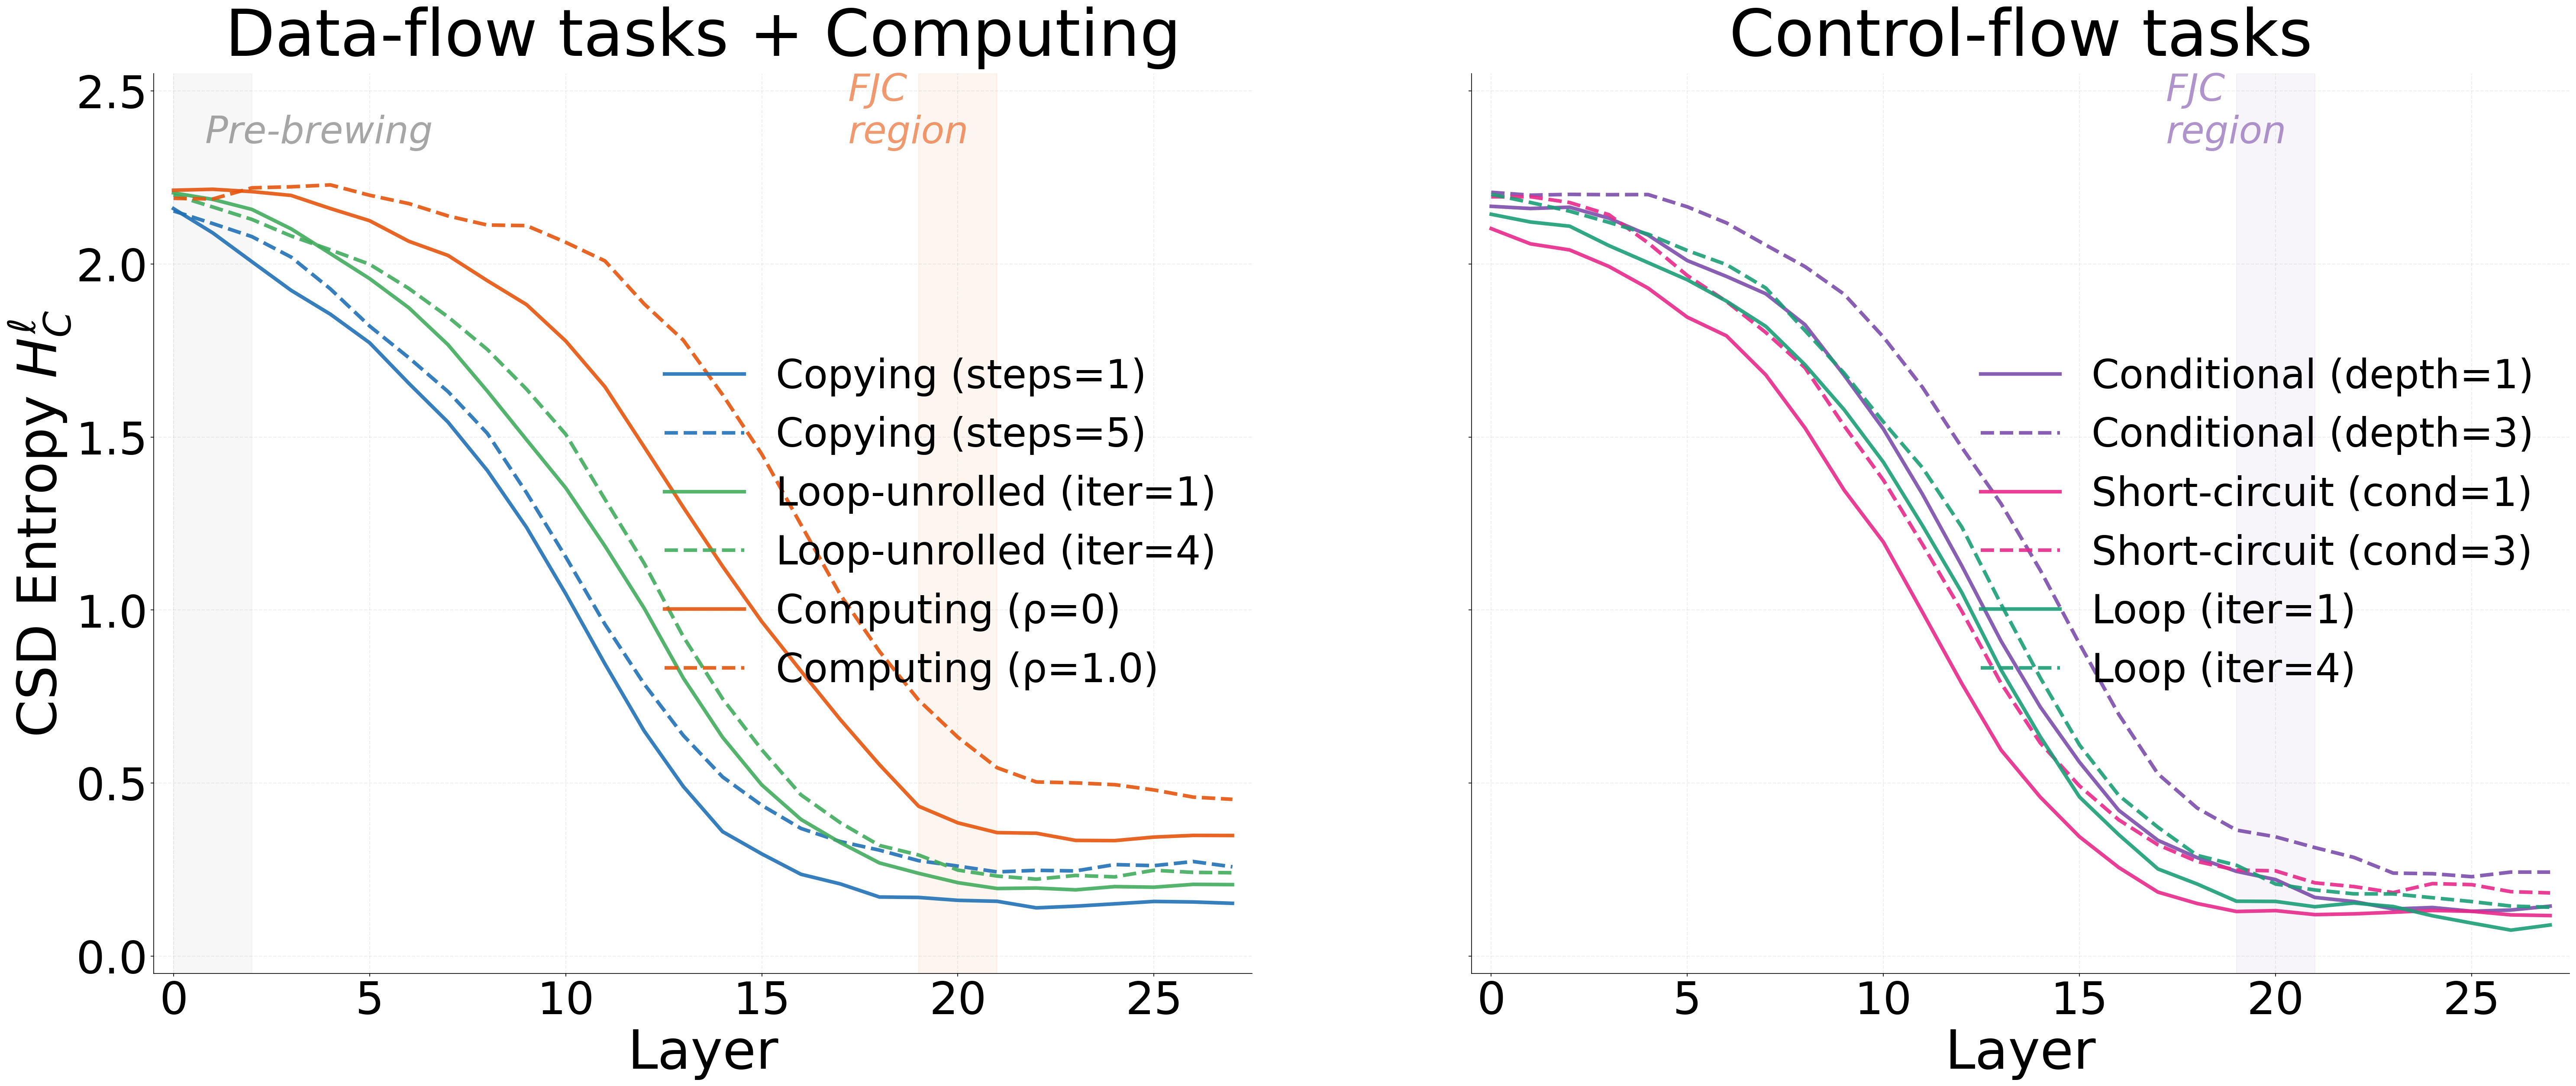
\includegraphics[width=\linewidth]{figures/appendix/G_brewing_dynamics_entropy.png}
\caption{Per-layer CSD entropy $H_C^\ell$ curves for each task at selected difficulty levels. The descent onset (related to FPCL) and convergence point (related to FJC) remain positionally stable; what varies is whether convergence is achieved.}
\label{fig:app:brewing_entropy}
\end{figure}

\begin{figure}[t]
\centering
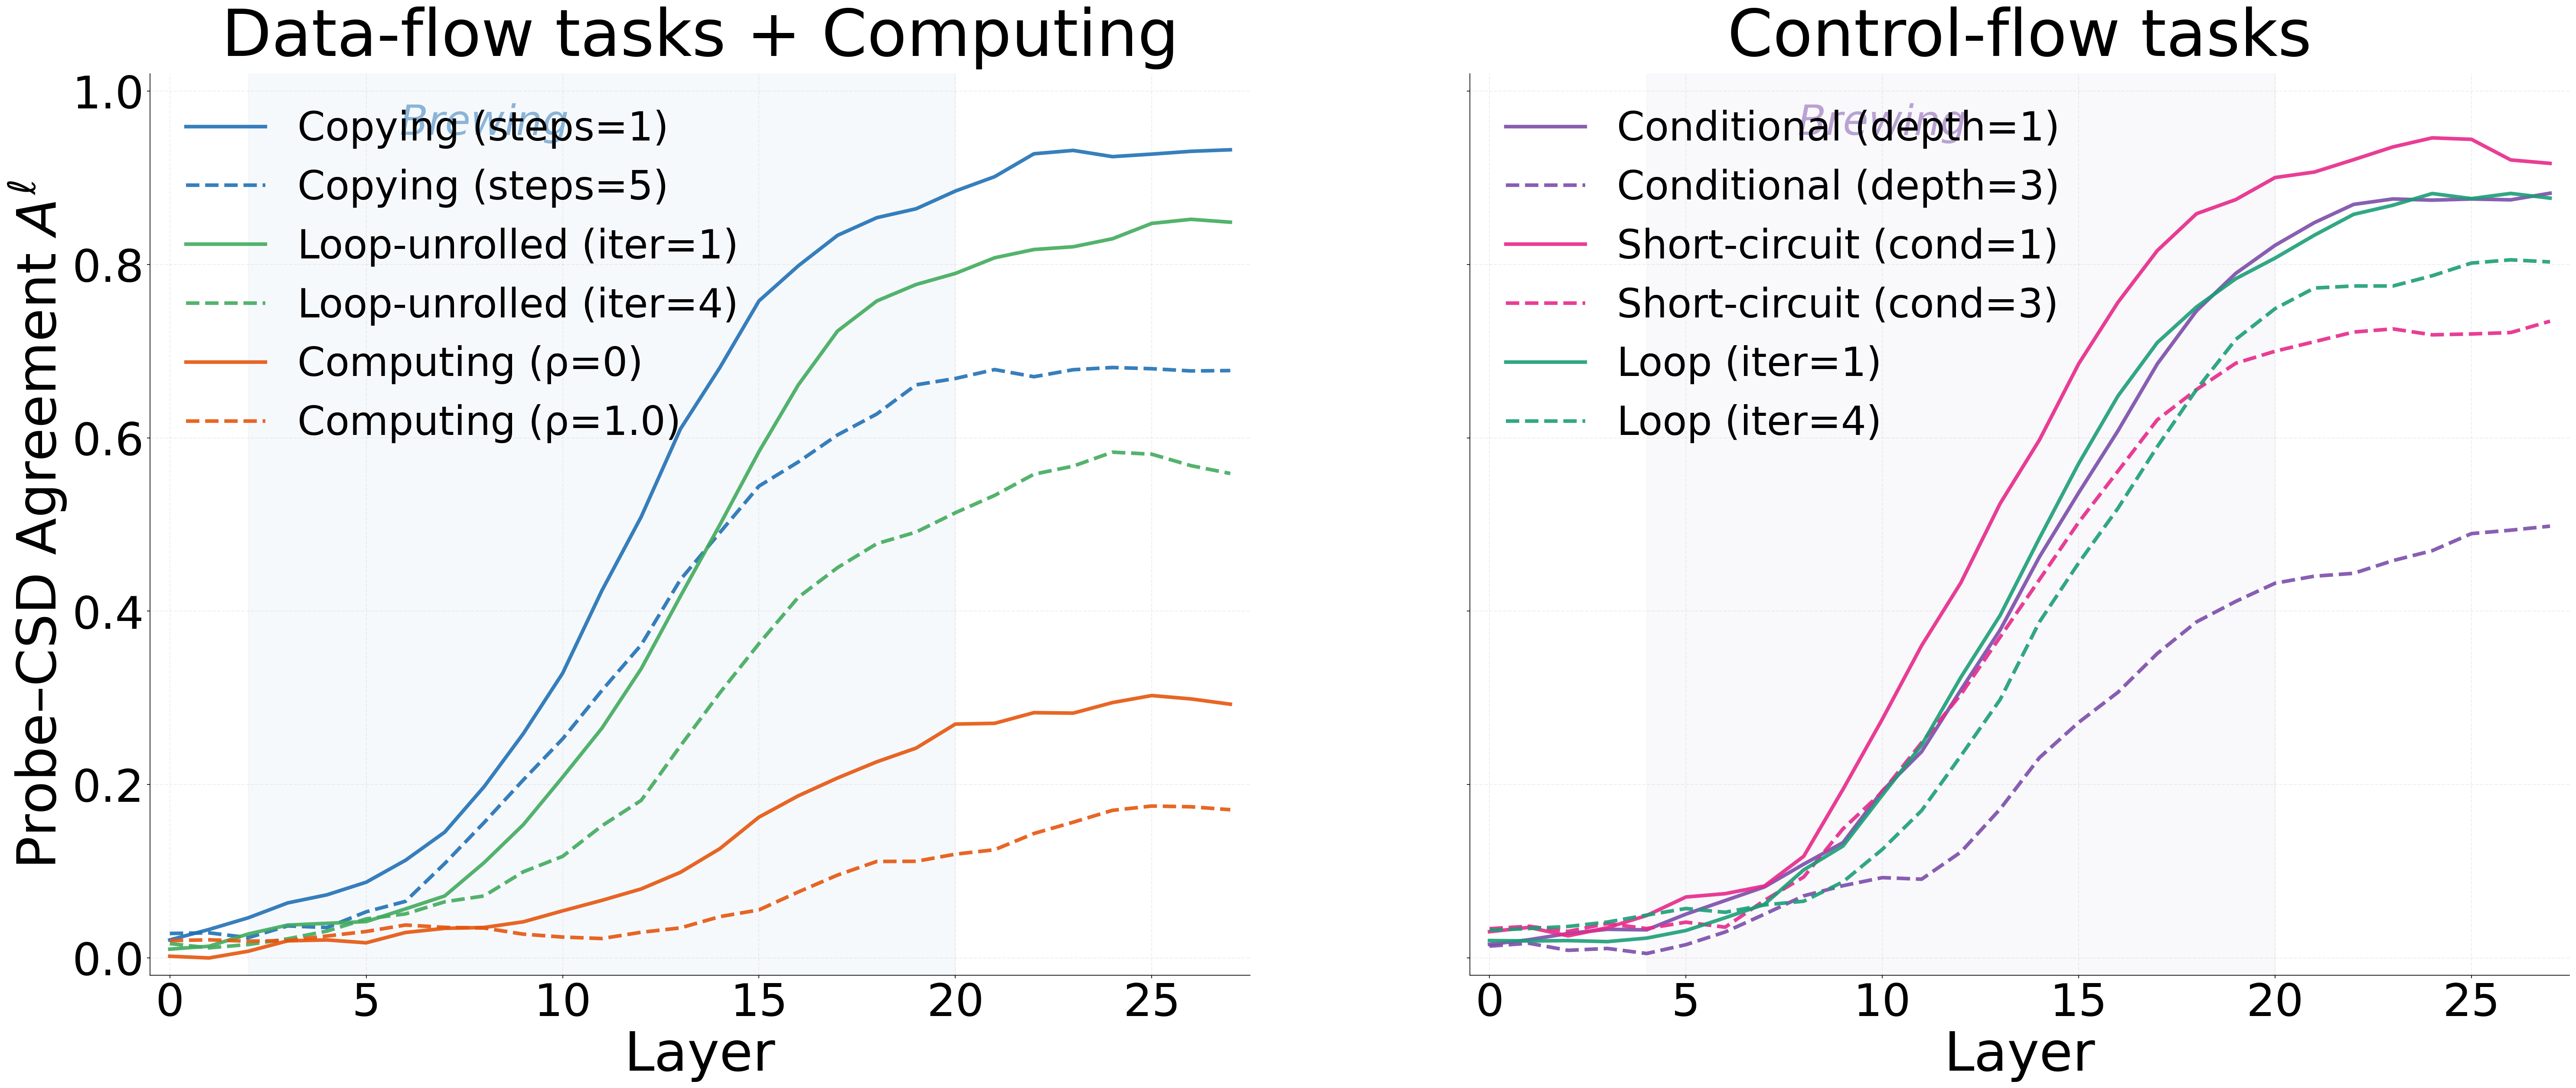
\includegraphics[width=\linewidth]{figures/appendix/G_brewing_dynamics_agreement.png}
\caption{Per-layer probe--CSD agreement $A^\ell$ trajectories for each task at selected difficulty levels. Agreement rises through the brewing phase and plateaus near FJC, with harder instances showing lower plateau values.}
\label{fig:app:brewing_agreement}
\end{figure}
